\documentclass[fleqn, a4paper, 12pt]{article}
%\setlength\parindent{0pt}
\usepackage[unicode]{hyperref}
\hypersetup{linktocpage}
\usepackage{graphicx}

\usepackage[final]{pdfpages}

\usepackage{selinput} 
\SelectInputMappings{
	adieresis={ä},
	germandbls={ß}
}
\usepackage[english]{babel}

\usepackage{setspace}
\setstretch{1.5}
\usepackage{tikz}
\usepackage[super]{nth}

\renewcommand{\underline}{\ul}

%math

\usepackage{amsmath, amssymb, amsfonts, amsthm, enumitem, stmaryrd, stmaryrd, mathrsfs}

\usepackage{sgame}

\newcommand{\rhs}{\mbox{RHS}}
\newcommand{\lhs}{\mbox{LHS}}

\newcommand{\degree}{^{\circ}}

% sets
\newcommand{\A}{\mathbb{A}}
\newcommand{\B}{\mathbb{B}}
\renewcommand{\C}{\mathbb{C}}
\newcommand{\D}{\mathbb{D}}
\newcommand{\K}{\mathbb{K}}
\renewcommand{\L}{\mathbb{L}}
\newcommand{\N}{\mathbb{N}}
\newcommand{\M}{\mathbb{M}}
\newcommand{\R}{\mathbb{R}}
\renewcommand{\S}{\mathbb{S}}
\newcommand{\Q}{\mathbb{Q}}
\newcommand{\Z}{\mathbb{Z}}

\newcommand{\yy}{\mathbb{Y}}
\newcommand{\xx}{\mathbb{X}}
\newcommand{\ww}{\mathbb{W}}

\newcommand{\snull}{\mathscr{N}}
\newcommand{\nullity}[1]{\mathrm{nullity} \left( #1 \right)}
\newcommand{\skern}{\mathscr{K}}
\newcommand{\lagr}{\mathscr{L}}
\newcommand{\mcol}[1]{\mathrm{col} \left( #1 \right)}
\newcommand{\colrk}[1]{\mathrm{colrank} \left( #1 \right)}
\newcommand{\mrow}[1]{\mathrm{row} \left( #1 \right)}
\newcommand{\rowrk}[1]{\mathrm{rowrank} \left( #1 \right)}

\newcommand{\gupp}[1]{\left\lceil #1 \right\rceil}
\newcommand{\glow}[1]{\left\lfloor #1 \right\rfloor}

\newcommand{\abs}[1]{\left\lvert #1 \right\rvert}
\newcommand{\eval}[1]{\left. #1 \right|}
\newcommand{\norm}[1]{\left\lVert #1 \right\rVert}

\renewcommand{\exp}[1]{\operatorname{exp} \left\{ #1 \right\}}
\renewcommand{\ln}[2][]{\operatorname{ln}^{#1} \left( #2 \right)}

\newcommand{\pr}[1]{\operatorname{Pr} \left( #1 \right)}

\newcommand{\e}[2][]{\mathbb{E}^{#1} \left[ #2 \right]}
\newcommand{\E}{\mathbb{E}}
\newcommand{\eu}[1]{\mathbb{EU} \left[ #1 \right]}
\newcommand{\cov}[1]{\mathbb{C}\mathrm{ov} \left( #1 \right)}
\newcommand{\var}[1]{\mathbb{V}\mathrm{ar} \left( #1 \right)}
\newcommand{\Var}{\mathbb{V}\mathrm{ar}}
\newcommand{\sd}[1]{\mathrm{SD} \left( #1 \right)}

\renewcommand{\log}[2][]{\operatorname{log}_{#1} \left( #2 \right)}
\renewcommand{\sin}[2][]{\operatorname{sin}^{#1} \left( #2 \right)}
\renewcommand{\cos}[2][]{\operatorname{cos}^{#1} \left( #2 \right)}
\renewcommand{\tan}[2][]{\operatorname{tan}^{#1} \left( #2 \right)}
\renewcommand{\sec}[2][]{\operatorname{sec}^{#1} \left( #2 \right)}

\newcommand{\tr}[1]{\operatorname{tr} \left( #1 \right)}
\newcommand{\adj}[1]{\operatorname{adj} \left( #1 \right)}
\newcommand{\sgn}[1]{\operatorname{sgn} \left( #1 \right)}
\newcommand{\vol}[1]{\operatorname{vol} \left( #1 \right)}
\renewcommand{\deg}[1]{\operatorname{deg} \left( #1 \right)}
\newcommand{\diag}[1]{\operatorname{diag} \left( #1 \right)}
\newcommand{\rank}[1]{\operatorname{rank} \left( #1 \right)}
\newcommand{\spec}[1]{\operatorname{spec} \left( #1 \right)}
\newcommand{\diam}[1]{\operatorname{diam} \left( #1 \right)}
\newcommand{\range}[1]{\operatorname{range} \left( #1 \right)}

\renewcommand{\vec}[1]{\operatorname{vec} \left( #1 \right)}

\newcommand{\vspan}[1]{\operatorname{span} \left\{ #1 \right\}}

\newcommand{\argmax}{\operatornamewithlimits{arg \, max}}
\newcommand{\argmin}{\operatornamewithlimits{arg \, min}}


\renewcommand{\d}{\, \mathrm{d}}
\newcommand{\nd}{\mbox{n.d.}}

% matrices
\newenvironment{mx}{\begin{matrix}}{\end{matrix}}
\newenvironment{bmx}{\begin{bmatrix}}{\end{bmatrix}}
\newenvironment{Bmx}{\begin{Bmatrix}}{\end{Bmatrix}}
\newenvironment{pmx}{\begin{pmatrix}}{\end{pmatrix}}
\newenvironment{vmx}{\begin{vmatrix}}{\end{vmatrix}}
\newenvironment{Vmx}{\begin{Vmatrix}}{\end{Vmatrix}}

% this allows for augmented matrices
\makeatletter
\renewcommand*\env@matrix[1][*\c@MaxMatrixCols c]{%
	\hskip -\arraycolsep
	\let\@ifnextchar\new@ifnextchar
	\array{#1}}
\makeatother
\usepackage{cleveref,booktabs}
% note: proof environment is pre-defined by amsmath
\crefname{proof}{Proof}{Proofs}

\theoremstyle{plain}

\newtheorem{theo}{Theorem}
\crefname{theo}{Theorem}{Theorems}

\newtheorem{lemm}{Lemma}
\crefname{lemm}{Lemma}{Lemmata}

\newtheorem{coro}{Corollary}
\crefname{coro}{Corollary}{Corollaries}

\newtheorem{prop}{Proposition}
\crefname{prop}{Proposition}{Propositions}

\newtheorem{conj}{Conjecture}
\crefname{conj}{Conjecture}{Conjectures}

\newtheorem{crit}{Criterion}
\crefname{crit}{Criterion}{Criteria}

\newtheorem{algo}{Algorithm}
\crefname{algo}{Algorithm}{Algorithms}


\theoremstyle{definition}

\newtheorem{defi}{Definition}%[section]
\crefname{defi}{Definition}{Definitions}

\newtheorem{cond}{Condition}
\crefname{cond}{Condition}{Conditions}

\newtheorem{prob}{Problem}[section]
\crefname{prob}{Problem}{Problems}

\newtheorem{exam}{Example}
\crefname{exam}{Example}{Examples}

\newtheorem{axio}{Axiom}
\crefname{axio}{Axiom}{Axioms}


\theoremstyle{remark}

\newtheorem{rema}{Remark}
\crefname{rema}{Remark}{Remarks}

\newtheorem{note}{Note}
\crefname{note}{Note}{Notes}

\newtheorem{nota}{Notation}[section]
\crefname{nota}{Notation}{Notations}

\newtheorem{term}{Terminology}[section]
\crefname{term}{Terminology}{Terminologies}

\newtheorem{clai}{Claim}
\crefname{clai}{Claim}{Claims}

\newtheorem{summ}{Summary}
\crefname{summ}{Summary}{Summaries}

\newtheorem{ackn}{Acknowledgment}[section]
\crefname{ackn}{Acknowledgment}{Acknowledgments}

\newtheorem{case}{Case}[section]
\crefname{case}{Case}{Cases}

\newtheorem{conc}{Conclusion}
\crefname{conc}{Conclusion}{Conclusions}


% others
\crefname{table}{Table}{Tables}
\crefname{figure}{Figure}{Figures}

\newcommand{\f}{\textbf}
\newcommand{\T}{\mathcal{T}}
\renewcommand{\S}{\mathcal{S}}
\newcommand{\nn}{\mathbb{N}}
\newcommand{\rr}{\mathbb{R}}
\newcommand{\siin}{\sum_{i=1}^{n}}
\newcommand{\siiin}{\sum_{i=1}^{\infty}}
\newcommand{\1}{\mathbb{1}_}
\newcommand{\am}{A^\prime\subseteq M^\prime}
\newcommand{\lp}{\mathfrak{L}_+}
\newcommand{\lin}{\lim\limits_{n\rightarrow\infty}}
\newcommand{\lini}{\liminf_{n\rightarrow\infty}}
\newcommand{\lins}{\limsup_{n\rightarrow\infty}}
\newcommand{\Iu}{\int u \text{ d } \mu}
\newcommand{\If}{\int f \text{ d } \mu}
\newcommand{\RV}{(\rr,\B)}
\newcommand{\RVE}{(\bar{\rr},\bar{\B})}
\renewcommand{\d}{\, \mathrm{d}}
\renewcommand{\G}{(G,\mathcal{S})}
\newcommand{\bce}{\text{Bayes correlated equilibrium}}
\newcommand{\is}{\text{information structure }}
\newcommand{\ins}{\text{individual sufficiency }}
\newcommand{\pl}{i \in \mathcal{I}}
\renewcommand{\a}{\alpha}
\renewcommand{\b}{\beta}
\usepackage{breakcites}
\newcommand{\m}{\mu_i}
\usepackage{color}
\usepackage{mathptmx}
\newcommand{\partition}[1]{
	\begin{tikzpicture}[scale=11]
	\draw (0, 0) -- (1, 0);
	\draw (0, .04) -- (0, -.04) node[below] {$0$};
	\draw (1, .04) -- (1, -.04) node[below] {$1$};
	
	\foreach \x/\label in {#1}
	\draw[very thick] (\x, .03) node[above] {\label} -- (\x, -.03) node[below] {$\x$};
	\end{tikzpicture}}
\begin{document} 
	1. First of all, let us short notation in terms of   $r_L:=r_{low}$ and $r_H:=r_{high}$. In order to check concavity of the objective function, consider its SOC: \begin{align*}
	\scriptstyle
-\gamma\,	p\, (w_0(1+r^f+\alpha(r_L-r^f)))^{-(1+\gamma)}\,(r_L-r^f)^2 +-\gamma\,(1-p)\, (w_0(1+r^f+\alpha(r_H-r^f)))^{-(1+\gamma)}\,(r_H-r^f)^2 
	\end{align*}
	Obviously its sign is ambiguous. Therefore, even though the (two) inequality constraints are (weakly) concave and  no  equality constraints arise, the first "convexity-condition" is not satisfied generally. That is,  KTK-conditions are just necessary (as usual) but not sufficient for an optimum.\\
	
	
	2. a)

FOC: \begin{align}\scriptstyle
p\, (w_0(1+r^f+\alpha(r_L-r^f)))^{-\gamma}\,(r_L-r^f) +(1-p)\, (w_0(1+r^f+\alpha(r_H-r^f)))^{-\gamma}\,(r_H-r^f)=0 
\end{align}
Assume the  opposite, i.e., that the optimal portfolio share $\alpha^*$ (the value of $\alpha$ for which  the equation above holds) depends on initial wealth $w_0$. Denote this maximizer contingent on $w_0$  by $\alpha(w_0)$. As the optimal portfolio share responds on $w_0$, the first order derivative of the LHS of (1) (setting $\alpha=\alpha(w_0)$) with respect to wealth should be equal zero. Namely, the total differentiation of the FOC w.r.t. $\alpha$ and $w_0$: \begin{align*} {\scriptstyle
\frac{\mathrm{d} \mathbb{E} \,u(w_1)}{\mathrm{d} \alpha \, \mathrm{d} w_0}=}&&\scriptstyle-\gamma \, w_0^{-(1+\gamma)} \, p\, (1+r^f+a(r_L-r^f))^{-\gamma}\,(r_L-r^f)+ w_0^{-\gamma} \,p \, \alpha'(w_0)\, (r_L-r^f)^2 & \\ && \scriptstyle-\gamma \, w_0^{-(1+\gamma)} \,(1-p)\, (1+r^f+a(r_H-r^f))^{-\gamma}\,(r_H-r^f)+ w_0^{-\gamma} \,p \, \alpha'(w_0)\, (r_H-r^f)^2 &\scriptstyle=0. \end{align*}
Clearly, this equality can be rearranged as follows: \begin{align*}&\scriptstyle w_0^{-\gamma} \,p \, \alpha'(w_0)\, (r_L-r^f)^2 +w_0^{-\gamma} \,p \, \alpha'(w_0)\, (r_H-r^f)^2 \\=&\scriptstyle\frac{1}{\gamma} \, w_0^{-(1+\gamma)} \, p\, (1+r^f+\alpha(r_L-r^f))^{-\gamma}\,(r_L-r^f)+\frac{1}{\gamma} \, w_0^{-(1+\gamma)} \,(1-p)\, (1+r^f+\alpha(r_H-r^f))^{-\gamma}\,(r_H-r^f)\intertext{and now, the RHS of this equality corresponds to the FOC multiplied by ${\gamma} \, w_0^{-1}$ which has to be still equal zero. Thus, dividing the  equality by the LHS (except $\alpha'(w_0)$) yields } & \alpha'(w_0)=\frac{0}{ w_0^{-\gamma} \,p \, (r_L-r^f)^2 +w_0^{-\gamma} \,p \, (r_H-r^f)^2}=0
\end{align*}    which contradicts that the optimal portfolio share depends on $w_0$.

Alternatively, notice that the initial objective (which we aim to maximize) can be divided by $w_0^\phi$ and  thus, wealth cancels out. Clearly, the optimal portfolio shares for the old resp. the new problem,  will coincide.\\

b) The associated FOC becomes: 
 \begin{align}  
  & \scriptstyle p\, (1+r^f+\alpha(r_L-r^f))^{\phi-1}\,(r_L-r^f) +(1-p)\, (1+r^f+\alpha(r_H-r^f))^{\phi-1}\,(r_H-r^f)=0 \intertext{using $(r_L-r^f)=-(r_H-r^f)=-0.1$ and rearranging we obtain }  & p^{\frac{1}{\phi-1}}\, (1+r^f+\alpha\,(-0.1)) =(1-p)^{\frac{1}{\phi-1}}\, (1+r^f+\alpha\, 0.1)\\ \Leftrightarrow & \, \,\alpha =10\, (1+r^f) \, \frac{ p^{\frac{1}{\phi-1}}-(1- p)^{\frac{1}{\phi-1}}}{ p^{\frac{1}{\phi-1}}+(1- p)^{\frac{1}{\phi-1}}}= 2.73308...
 \end{align}
 evaluated at $p=0.1$, $r^f=0.02$ and $\phi=-3$.\\
 
 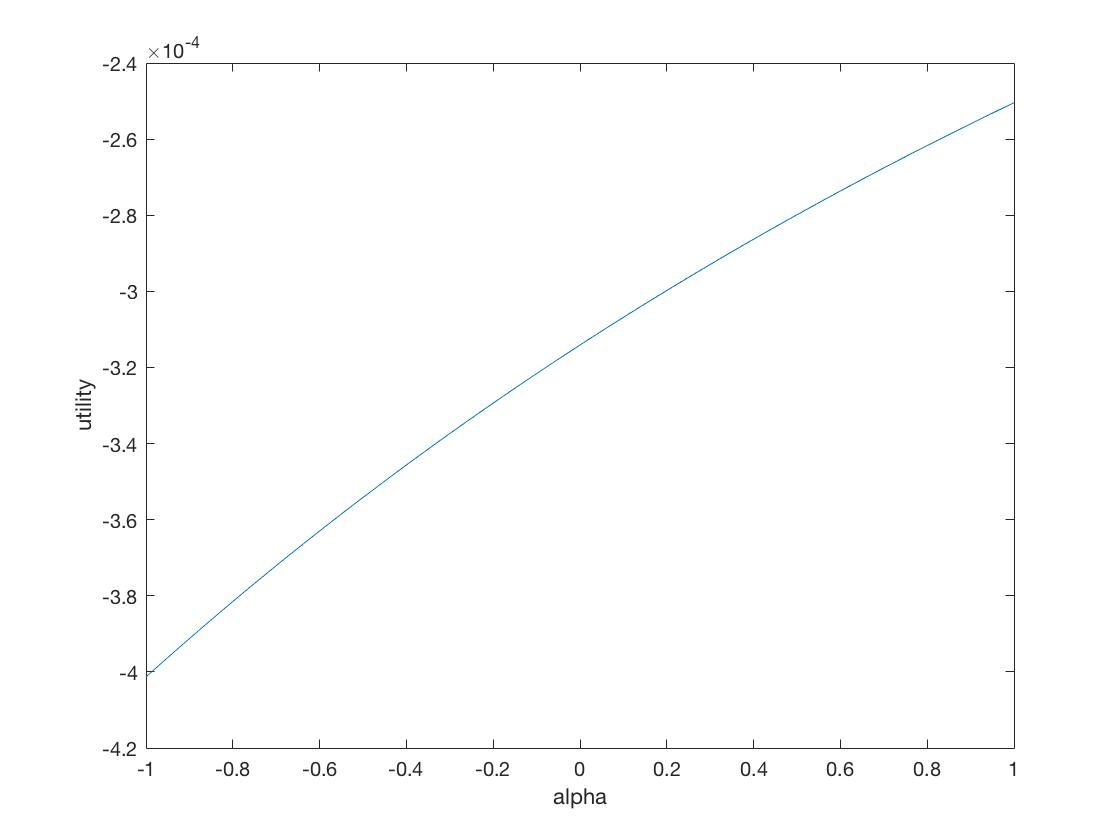
\includegraphics[width=\textwidth,height=\textheight,keepaspectratio]{PS3Q5Sub2.jpg}
 
3. a) Intuitively , $\alpha\geq 0$ prevents the case where the household  supplies the portfolio and  $\alpha\leq 1$ rules out that  the household borrows money in order to invest more in the portfolio.


\end{document}